%%% File encoding: UTF-8
%%% äöüÄÖÜß  <-- keine deutschen Umlaute hier? UTF-faehigen Editor verwenden!

%%% Magic Comments zum Setzen der korrekten Parameter in kompatiblen IDEs
% !TeX encoding = utf8
% !TeX program = pdflatex 
% !TeX spellcheck = de_DE
% !BIB program = biber

\documentclass[bachelor,german,smartquotes]{hgbthesis}
% Zulässige Optionen in [..]: 
%   Typ der Arbeit: 'diploma', 'master' (default), 'bachelor', 'internship' 
%   Hauptsprache: 'german' (default), 'english'
%		Turn on smart quote handling: 'smartquotes'
%	  Use APA bibliography style: 'apa'
%%%----------------------------------------------------------

\RequirePackage[utf8]{inputenc}		% bei der Verw. von lualatex oder xelatex entfernen!

\usepackage[parfill]{parskip}

% uspackage below is for listing name of formula's variables
\usepackage{array,tabularx}
\newenvironment{conditions*}
{\par\vspace{\abovedisplayskip}\noindent
	\tabularx{\columnwidth}{>{$}l<{$} @{\ : } >{\raggedright\arraybackslash}X}}
{\endtabularx\par\vspace{\belowdisplayskip}}

% wrapping log words
\newcolumntype{P}[1]{>{\hspace{0pt}}p{#1}}

% TODO: \usepackage{graphicx} required

\graphicspath{{images/}}    % Verzeichnis mit Bildern und Grafiken
\logofile{logo}							% Logo-Datei = images/logo.pdf (\logofile{}, wenn kein Logo gewünscht)
\bibliography{references}  	% Biblatex-Literaturdatei (references.bib)

%%%----------------------------------------------------------
% Angaben für die Titelei (Titelseite, Erklärung etc.)
%%%----------------------------------------------------------

%%% Einträge für ALLE Arbeiten: -----------------------------
\title{Algorithmen für verteilte Systeme in unbemannten Luftfahrzeugen}
\author{Artsiom Kaliaha}

%\programtype{Fachhochschul-Bachelorstudiengang}		% select/edit
\programtype{Fachhochschul-Bachelorstudiengang}

\programname{Automotive Computing}
\placeofstudy{Hagenberg}
\dateofsubmission{2021}{02}{01}	% {YYYY}{MM}{DD}

\advisor{Mag. Dipl.-Ing. Dr. Andreas Müller B.Sc.}	% optional

%\strictlicense		%%% restrictive license instead of Creative Commons (discouraged!)

%%%----------------------------------------------------------
\begin{document}
%%%----------------------------------------------------------

%%%----------------------------------------------------------
\frontmatter                    % Titelei (röm. Seitenzahlen)
%%%----------------------------------------------------------

\maketitle
\tableofcontents

%\chapter{Vorwort}

 				% Vorwort ist optional
\chapter{Kurzfassung}


Drohnen ändern den Alltag auf überraschende Weise: sie retten in Katastrophengebieten, sichern die medizinische Versorgung in Konfliktzonen, reduzieren Verkehr und Emissionen und machen riskante Berufe sicherer. Andere Gebiete, bei denen Drohnen zum Einsatz kommen, sind das Militär (Steuerung von Drohnenschwärmen), der Telekommunikationsbereich (schneller Aufbau von Netzwerken auf Nachfrage) und die Ausbildung (Aufnahme von 360-Grad-Videos).

Es gibt mehrere Forschungsrichtungen, die Funktionsweise einzelner Drohnen und Drohnenschwärmen optimieren. Eine von dennen ist Swarming. Swarming (bzw. Schwarmintelligenz) ist ein Bereich von Multiagentensystem, der Drohnen ermöglicht, bestimmte Tierarten nachzuahmen. Die Schwarmintelligenz ermöglicht es hunderten, wenn nicht tausenden von Drohnen, zusammenzuarbeiten, um herausfordernde Aufgaben zu erledigen. 

Heutzutage forscht die gesamte Robotikindustrie auf dem Gebiet der kollaborativen Robotik, bei der Roboter nebeneinander arbeiten und von Menschen trainiert werden. Schon in Naher Zukunft werden wir aber in der Zeit der Cloudrobotik leben, in der Roboter ohne menschlicher Interaktion als ein einziger Organismus agieren und denken werden. Fortschritte in den Bereichen der Künstlicher Intelligenz und der Cloudrobotik treiben die Schwarmtechnologie an und werden dazu beitragen, dass Drohnen nicht nur mit ihren Operatoren, sondern auch miteinander kommunizieren werden. Heutzutage wird jede Drohne von einem oder mehreren Menschen gesteuert. Die Drohnen von morgen werden möglicherweise überhaupt keine Operatoren brauchen. Forscher untersuchen Möglichkeiten, Menschen durch Künstliche Intelligenz und Algorithmen für verteilte Systeme zu ersetzen. Da eingebettete Systeme mit jedem Jahr leistungsstärker werden, haben sie genug Kapazitäten, um Sensordaten ohne Cloudverbindung zu bearbeiten, Rechenoperationen gleichmäßig untereinander aufzuteilen und Drohnen mit speziellen Funktionen im Schwarm redundant abzusichern. 

Alle diesen Funktionen brauchen klassische Algorithmen für verteilte Systeme, die schon seit Jahren bei Cloudlösungen zum Einsatz kommen. Sie beruhen auf den Algorithmen aus den 80ern und 90ern, die immer noch in Produktivsystemen verwendet werden und als Inspiration für neue und optimalere Algorithmen dienen. Der Fokus dieser Bachelorarbeit liegt auf der Untersuchung verfügbarer Algorithmen für verteilte Systeme und auf der Recherche nach einem optimalen Concurrency Modell für robuste und fehlertolerante eingebettete Systeme.
		
\chapter{Abstract}


\begin{english} %switch to English language rules

Drones change everyday life in surprising ways: they save in disaster areas, provide medicine in conflict zones, reduce traffic flow and emissions, and make risky jobs safer. Today, drones are used in many ways. Other areas where drones are used are the army (control of swarms of drones), the telecommunications sector (on demand network provisioning) and training (360-degree videos).

There are several research areas that focus on optimizing individual drones operation and swarms of drones control. One of these research topics is swarming. Swarming is a subfield of multi-agent systems that allows drones to mimic behavior of certain animal species. Swarm intelligence allows hundreds, if not thousands, of drones to work together to complete challenging tasks. 

Today the entire robotics industry is doing research in the field of collaborative robotics, which enables robots to work side by side with humans and to be trained by humans. In the near future, however, we will be living in the age of cloud robotics, in which robots will act and think as a single organism without human interaction. Advances in artificial intelligence and cloud robotics are driving swarm technology and will help drones communicate not only with their operators, but also with each other. Nowadays, each drone is controlled by one or more people, but drones may not need operators at all. Researchers are investigating possibilities of replacing humans with artificial intelligence and algorithms for distributed systems. As embedded systems become more powerful each year, they get more and more capacity to process sensor data without cloud connection. Innovative approaches to building swarm systems suggest splitting computation evenly across all drones and redundantly securing drones which fulfill special functions in a swarm or carry unique hardware.

All of these functions require classic algorithms for distributed systems that were used in cloud solutions for years. They are based on the algorithms from the 80s and 90s, which are still used in production systems and serve as inspiration for more optimal algorithms. The goal of this bachelor thesis is to investigate available algorithms for distributed systems and find an optimal concurrency model for robust and fault-tolerant embedded drone systems.


\end{english}

			

%%%----------------------------------------------------------
\mainmatter          % Hauptteil (ab hier arab. Seitenzahlen)
%%%----------------------------------------------------------

\chapter{Einleitung}
\label{cha:Einleitung}

Wir leben in der Zeit der künstlichen Intelligenz \cite{MITai}, Big Data \cite{MITbigData, MITbigData2} und der intelligenten Robotersysteme \cite{MITrobots, MITrobots2}. Heutzutage ist die Vielfalt der Robotersysteme sehr beeindruckend: Roboter finden Einsatz in Form autonomer Autos, intelligenter Produktionstechnik und auch \textit{Drohnen}. Vor 5 Jahren waren Drohnen noch manuell gesteuert, und erlaubten keine anspruchsvolle Rechenoperationen direkt auf der Hardware. Zukünftig sollen Drohnen leistungsfähiger sein und noch autonomer funktionieren und das nicht nur einzeln sondern auch in Schwärmen. Der Fokus dieser Arbeit liegt im Gebiet der Drohnenschwärme, genauer gesagt in der Betrachtung dieser als \textit{verteilte Systeme}. Dadurch, dass Drohnen miteinander kommunizieren, können sie in einem Schwarm voll autonom und ohne Kollisionen fliegen. Die Kommunikation im Schwarm liefert in diesem Fall zusätzliche Informationen für die Funktion des autonomen Fliegens. Ein weiterer möglicher Anwendungsfall ist die Entlastung von Operatoren, die diese Drohnen normalerweise steuern. Die Entwicklung von Drohnen mit einem hohen Grad an Autonomie bietet den Operatoren im Laufe einer Mission bzw. eines Auftrages mehr Freiheit, andere nützliche Aufgaben zu erfüllen (Kamera ausrichten, Objekt beobachten, 3D Mapping des Geländes steuern, usw).

Fortschritte in Kommunikationstechnologien (vor allem 5G), Künstlicher Intelligenz und eingebetteter Hardware haben die zweite Welle von \textit{Drohnentechnologie} ausgelöst. Manche Anwendungsfälle, die früher nicht denkbar waren, werden derzeit in Forschungsinstituten und Universitäten (in Europa vor allem EPFL  \footnote{Die École polytechnique fédérale de Lausanne ist eine technisch-naturwissenschaftliche Universität in Lausanne, Schweiz.} und ETH Zürich) erforscht. Innovative Startups versuchen, all diesen Anwendungsfälle auf den Markt zu bringen. Die Drohnenindustrie bietet bahnbrechende Anwendungsfälle und dadurch auch neue Herausforderungen.

Das Problem, das diese Arbeit löst, befasst sich mit einer solchen Herausforderung, und zwar \textit{der Synchronisation zwischen mehreren Knoten in einem Cluster von Drohnen}. Wenn Drohnen eine abstrakte Kommunikationstechnologie verwenden, muss ein Algorithmus gewählt werden, der Daten von Drohnen in einem Schwarm zuverlässig synchronisiert. Um eine passende Lösung dafür zu finden, wurden bestimmte Algorithmen verglichen. Zwei Algorithmen, die sich bei der Betrachtung verteilter Systeme und der Synchronisation von Konten besonders auszeichnen, sind \textit{Paxos} und \textit{Raft}. Das Problem der Synchronisation zwischen den Knoten eines Systems wird in der Informatik auch \textit{"Problematik der Replikation des Zustandsautomaten"} genannt. Langjährige Erfahrungen der Cloudprovider, die diese Algorithmen für mehrere Bereiche ihrer Infrastruktur einsetzen (vor allem Speicherdienste und \textit{MapReduce} \footnote{MapReduce ist ein Programmiermodell für nebenläufige Berechnungen über große Datenmengen auf Computerclustern.} Clusters), haben die Nutzbarkeit dieser Algorithmen bewiesen. Zwar werden beide Algorithmen in zahlreichen Produktivsystemen benötigt, die Meinungen über die jeweiligen Stärken und Schwächen der Algorithmen sind jedoch noch gespalten.

In einem engen Zusammenhang mit verteilten Systemen stehen \textit{Concurrency Modelle}. Ergänzend zu den unabhängigen Fehlern der Teilkomponenten und dem Fehlen der Global Clock ist die Concurrency eine der wichtigsten Eigenschaften der verteilten Systeme. In dieser Bachelorarbeit werden die Eigenschaften mehrerer Concurrency Modelle verglichen, um ein dafür am besten geeignetes Modell für die Entwicklung verteilter Systeme zu finden.

Überblick über das Dokument: im 2. Kapitel~\ref{cha:Analyse} wird das Thema der Drohnen und der Interaktion von Drohnen in einem Schwarm betrachtet: was sind die Vor- und Nachteile bei der Verwendung eines Schwarms, welche Schwierigkeiten bringt die Steuerung eines Schwarms mit sich, welche theoretischen Frameworks gibt es für die Steuerung verteilter Agenten. Außerdem wird das Thema der verteilten Systeme behzandelt: theoretische Grundlagen werden erläutert und Algorithmen für verteilte Systeme verglichen. Anschließend werden Concurrency Modelle für die Implementierung verteilter und ausfallsicherer Systeme untersucht. Das letzte Kapitel der Arbeit~\ref{cha:Entwicklung} befasst sich mit der Umsetzung eines der besprochenen Algorithmen mit einem der ausgewählten Concurrency Modelle. In diesem Kapitel wird der ausgewählte Algorithmus im Detail analysiert und erklärt. Welche Entscheidungen wurden bei der Umsetzung getroffen und weshalb. Zudem zeigt dieses Kapitel, welche Vorteile die ausgewählten Werkzeuge bieten.

\chapter{Analyse}
\label{cha:Analyse}

Um die Problemstellung der Arbeit besser zu verstehen, muss man einige grundlegende Konzepte der \textit{Schwarmrobotik} und verteilter Systeme verstehen. Außerdem gibt dieses Kapitel einen Überblick auf den aktuellen Stand der Technik, Optionen und Empfehlungen für technische Umsetzung.

\section{Vorteile von Drohnenschwärmen}

Heutzutage werden Drohnen entweder einzeln verwendet oder sie finden in einem Drohnenschwarm ihre Anwendung. Beide Verwendungsarten haben Vor- und Nachteile und umfassende Anwendungsfälle. Um den Weg von einer Drohne zu einem Drohnenschwarm zu verstehen, muss man zuerst die Forschungsrichtungen im Feld von UAVs (Unmanned Aerial Vehicles) betrachten. Zu UAVs gibt es vier Forschungsschwerpunkte, die an entsprechende Herausforderungen gebunden sind:

\begin{enumerate}
	\item Ein einziges UAV muss stets in der Lage sein, bestimmte Gebiete und Flächen zu überfliegen.
	\item Objekte und Ereignisse von Interesse müssen von dem UAV erkannt werden können.
	\item Um einen Synergieeffekt zu erreichen, ist die Kommunikation zwischen mehreren Drohnen essenziell.
	\item Damit das Arbeiten der Drohnen an einem gemeinsamen Ziel ermöglicht wird, gilt es die Koordination eines Netzwerks von UAVs zu ermitteln.
\end{enumerate}

Diese Bachelorarbeit fokussiert sich auf Drohnenschwärme und auf die Koordination zwischen den einzelnen Drohnen. Betrachtet man eine Gruppe von Drohnen, stellt man fest, dass man einen Algorithmus benötigt, der die Funktionsweise dieser Gruppe optimiert, damit diese durch Zusammenarbeit ein gemeinsames Ziel erreicht. Unter anderem können folgende Probleme durch die Anwendung eine Schwarms gelöst werden:

\begin{description} 
	\item[Verteilung von Rechenoperationen (optimale Nutzung von Ressourcen).] Das ist ein klassischer Anwendungsfall aus der Informatik. Keine einzelne Drohne hat genug Rechenleistung, um eine schwierige Operation im Stand-Alone-Betrieb bzw. ohne Verbindung zur Cloud zu berechnen. Dadurch, dass es in einem Schwarm mehrere Drohnen gibt, kann die Arbeit aufgeteilt werden. So einen Ansatz kann man “Ad-Hoc Cloud” nennen. Unter der optimalen Nutzung von Ressourcen kann man auch den Austausch von lokalen Karten und Sensorwerten verstehen.
	
	\item[Verteilung von Aufgaben.] Für eine bestimmte Art von Problemen, die Schwarmintelligenz zur Lösung benötigt, ist es wünschenswert, dass jede Drohne eine bestimmte Funktion übernimmt und durch ihre speziellen Fähigkeiten (künstliche Intelligenz) oder Ausrüstung (Sensoren und Aktuatoren) hilft, das gemeinsame Ziel zu erreichen.
	Aus der Sicht der Ausfallsicherheit, Robustheit und Zuverlässigkeit eines verteilten Systems ist es immer besser, Tasks auf mehrere Geräte zu verteilen.  Dieser Zusammenhang wurde schon durch die Erfahrungen von Google mit verteilten Systemen bewiesen. Andererseits muss man mit dem Kommunikationsoverhead und der gestiegenen Komplexität bei der Entwicklung rechnen.
	
	\item[Ausfallsicherheit.] Ein Drohnenschwarm ist robust gegen Teilausfälle und bietet mehr Flexibilität bei Missionen. Wie oben schon erwähnt, können Aufgabenbereiche auf einzelne Drohnen und Drohnengruppen aufgeteilt werden.
	
	\item[Kollektive Entscheidungsfindung.]	Jede Drohne im Schwarm kann bzw. darf nur einen Teil vom ganzen Problem kennen. Für die Entscheidungsfindung braucht ein automatisiertes System sehr häufig nicht nur das lokale Wissen, sondern auch die Vogelperspektive oder den “Meinungsaustausch” mit anderen Drohnen.
\end{description}

\section{Autonomie im Drohnenschwarm}

Die im vorherigen Subkapitel erwähnten Vorteile eines Schwarms werden von Softwarekomponenten einer Drohne definiert, da diese Softwarekomponenten das Kommunikationsmuster bestimmen. Ein wichtiger Aspekt dabei ist die Autonomie von Drohnen. Autonomie ermöglicht einzelne Drohnen eines Schwarms lokale Entscheidungen zu treffen. 

\subsection{Methoden zur Kommunikation im Drohnenschwarm}

Um die Vorteile, die Autonomie einzelner Drohnen mit sich bringt, ausnutzen zu können, können folgende systematische Ansätze angewendet werden:

\begin{description} 
	\item[Multiagentensystem.] Ein Multiagentensystem ist eine Klasse von Algorithmen, in der einzelne Agenten basierend auf vordefinierten Regeln und Einschränkungen miteinander interagieren. Dadurch wird ein kollektives Verhalten ermöglicht.
	
	Die Interaktionen im System finden sowohl zwischen Agenten untereinander als auch zwischen Agenten und der Umgebung statt. Dabei spielt die sogenannte \textit{"Reward Function"} eine wichtige Rolle. Diese beschreibt, wie sich ein Agent verhalten muss. Der \textit{"normative Inhalt"} schreibt dem Agenten vor, wie er bestimmte Aufgaben lösen soll. Im Multiagentensystem kennt ein Agent den gesamten Problembereich bzw. -raum  nicht und muss die Lösung deswegen durch Lernen herausfinden. Multiagentensysteme üben Selbstorganisation, komplexe Verhaltensweisen und auch Kontrollparadigmen aus, obwohl individuelle Strategien von allen Agenten einfach sind.
	
	Ein Agent im Multiagentensystem hat einige wichtige Eigenschaften: \textit{Autonomie} (ein Agent ist teilweise unabhängig, selbstbewusst und autonom), \textit{lokaler Überblick} (kein Agent hat einen globalen Überblick und das System ist für einen einzelnen Agent zu komplex) und \textit{Dezentralisierung} (kein Agent wird als Leader bezeichnet / gewählt).
	
	\item[Verteilte Problemlösung.] Kooperative verteilte Problemlösung ist ein Netzwerk von halbautonomen Verarbeitungsknoten, die zusammenarbeiten, um ein Problem zu lösen. Dabei geht es um die Untersuchung der Problemaufteilung, Unterproblemaufteilung, Synthese vom Ereignis, Optimierung des Problemlösers und Koordination. Es ist eng mit der verteilten Programmierung und der verteilten Optimierung verbunden.
	
	In der verteilten Problemlösung arbeiten mehrere Agenten daran, ein spezifisches Problem zu lösen. Das wichtigste in diesen Systemen ist, dass Kooperation erforderlich ist, weil kein einziger Agent genug Informationen, Wissen und Fähigkeiten hat, um das Problem zu lösen. Die eigentliche Herausforderung besteht in der Sicherstellung, dass die Informationen so aufgeteilt werden, dass die Agenten einander ergänzen und nicht miteinander im Konflikt stehen. Ein Algorithmus für die verteilte Problemlösung muss ein größeres Problem in Teilaufgaben unter Berücksichtigung der räumlichen, zeitlichen oder funktionalen Aspekte gliedern.
	
	Ein Algorithmus für verteilte Problemlösung muss unter folgenden Einschränkungen handeln:
	\begin{enumerate}
		\item Kein Knoten hat genug Informationen, um das Problem selbstständig zu lösen.
		
		\item Im System gibt es weder eine globale Steuerung, noch einen Speicher. Steuerung und Speicher sind verteilt.
		
		\item Die Berechnung von Operationen auf einer lokalen CPU ist grundsätzlich schneller und weniger aufwändig als die Aufteilung derselben Operationen auf verteilte Systeme.
		
		\item Darüber hinaus muss das zu lösende Problem modular sein. Außerdem darf es keinen einzigartigen Knoten geben, da dies zu einem \textit{Bottleneck} im System führen kann. Ein solcher \textit{einzigartiger Knoten} wäre jener, der im Cluster oder im Schwarm eine spezielle Rolle erfüllt. Eine solche Aufgabe könnte beispielsweise die eines Leaders oder eines Koordinators sein.
	\end{enumerate}
	
	
	\item[Schwarmintelligenz / Schwarmrobotik.] Schwarmintelligenz ist das kollektive Verhalten von dezentralisierten, selbstorganisierten, natürlichen oder künstlichen Systemen. Das Konzept wird sehr oft im Bereich der Künstlichen Intelligenz eingesetzt.
	
	Systeme mit Schwarmintelligenz bestehen typischerweise aus einer Population von Agenten und Boids, die untereinander und mit der Umgebung kommunizieren. Inspiration für solche Systeme kommt aus der Natur, vor allem aus biologischen Systemen. Die Agenten folgen sehr einfache Regeln. Obwohl es keine zentralisierte Steuerung gibt, führen lokale und bis zu einem gewissen Grad zufällige Interaktionen zur Entstehung eines intelligenten und globalen Verhaltens. Ein klassisches Beispiel aus der Natur sind Ameisenkolonien.
	
	An dieser Stelle sieht man, dass die Grenzen zwischen Multiagentensystem, verteilter Problemlösung und Schwarmintelligenz verschwimmen können. In der Tat ist das Bilden einer klaren Grenze sehr schwierig.
\end{description}

\subsection{Einblick in zukünftige Systeme}

Moderne Systeme sind meist mit der Cloud verbunden oder brauchen zumindest eine kurze Synchronisation mit einem Cloud-Server. Nehmen wir an, dass eine Drohne eine Mission erfüllen soll, was sowohl Kommunikation zwischen Drohnen als auch zwischen dem Schwarm und der Cloud erfordert. Alle eingebetteten Systeme sind bis zu einem gewissen Grad in ihren Ressourcen (Rechenleistung, Akku, Konnektivität, Speicher) eingeschränkt. Dennoch wäre es sinnvoll, \textit{Missionsinformationen} zwischen der Cloud und einer einzelnen Drohne (dem sogenannten Leader) zu synchronisieren und mittels eines Algorithmus im Schwarm zu verteilen.

Dies widerspricht dem Regel, dass jeder einzigartige Knoten in einem verteilten System ein potenzielles Bottleneck ist, da die Präsenz eines speziellen Knotens die Durchsatzrate senken und die Ausfallsicherheit des Gesamtsystems verringern kann. Diese Herausforderungen müssen natürlich mit einem klugen Algorithmus ausgeglichen werden, womit sich diese Arbeit auch befasst.

In der Zukunft sollen Systeme wie Drohnenschwärme selbstorganisierend und autonom agieren. Laut den Forschungsergebnissen der Technischen Hochschule Lausanne (EPFL) sind allerdings mit aktuellem Stand der Technik in der Robotik 100\% selbstorganisierende Systeme weniger effizient als die Systeme, in denen Kommunikation zwischen Knoten möglich ist. Das heißt, dass die Synchronisation von Knoten im Schwarm eine gültige und in der Branche durchaus akzeptierte Lösung ist.

\section{Analyse von Algorithmen für verteilte, ausfallsichere Systeme}

Wie bereits im vorherigen Kapitel festgestellt, ist für das Funktionieren eines Schwarms die \textit{Replikation} von Daten zwischen den Knoten erforderlich. Diese Aufgabe umfasst das Themengebiet der verteilten Systeme. Die Auswahl eines Algorithmus beeinflusst die Robustheit des Gesamtsystems und wird in diesem Kapitel betrachtet.

Verteilte Systeme finden in mehreren Teilen der IT-Infrastruktur Einsatz. Häufige Einsatzbereiche sind:

\begin{enumerate}
	\item Dateisysteme
	
	\item Datenbanken
	
	\item Key-Value Stores (Schlüssel-Werte-Datenbank oder eine verteilte Hashtabelle)
	
	\item Queues (Verarbeitung von Datenströmen, keine einfache Datenstruktur in diesem Kontext)
\end{enumerate}

Diese genannten Systeme haben zwar unterschiedliche Anwendungsgebiete, die potenziell auftretenden Probleme sind allerdings sehr ähnlich:

\begin{description} 
	\item[Fehlertoleranz.] Um die Fehlertoleranz zu garantieren, muss ein System mehrere \textit{Replica} aller Daten besitzen und beim Ausfall der \textit{Hauptreplica} auf eine andere reibungslos und ohne Datenverlust umsteigen können. Die Anzahl von Replicas soll immer eine ungerade Zahl sein, typischerweise werden drei oder fünf Replicas gebildet. Eine ungerade Zahl verhindert eine gleiche Aufteilung von Stimmen zwischen 2 Gruppen von Replicas. Gibt es eine Mehrheit aller Knoten, die den gleichen Wert haben, werden diese Daten als korrekt gewertet.
	
	\item[Zeit für Wiederherstellung.] Ein Algorithmus für das verteilte System muss die Zeit für die Wiederherstellung verkürzen und intelligent auf mögliche Ausfälle reagieren. Der Algorithmus muss das Cluster unter neuen Einschränkungen umstrukturieren.
	
	\item[Erreichbarkeit.] Die Erreichbarkeit eines Systems stellt fest, ob ein Knoten als abgestürzt oder als laufend betrachtet werden soll. In verteilten Systemen gibt es allerdings keine Möglichkeit zu überprüfen, ob ein Knoten abgestürzt ist oder das Netzwerk dieses Knotens überfordert ist. In modernen Systemen wird das Problem mittels \textit{Timer} gelöst. Nach einem bestimmten Timeout wird der Knoten als nicht mehr erreichbar markiert. Nach welcher Zeit ein Knoten als nicht erreichbar betrachtet wird, ist für jede Konfiguration des Clusters spezifisch.
	
	\item[Skalierbarkeit und Durchsatzrate.] Die Skalierbarkeit und Durchsatzrate in verteilten Systemen wird durch “Scaling up” Verfahren erreicht, wenn zur Lösung eines Problems oder für eine bessere Fehlertoleranz mehrere Knoten zusammengebracht werden. Für ein klassisches “Scaling up” Verfahren braucht man dagegen einen neuen, leistungsfähigeren Rechner, der alle Anfragen abarbeiten kann. Eine weitere Lösungsmöglichkeit stellen Algorithmen dar. Ein Algorithmus, der Leseoperationen von allen Knoten eines Clusters erlaubt, ist viel effizienter als der Algorithmus, der Leseoperationen nur von einem einzigen Knoten im Cluster erlaubt. Dieser einzige Knoten ist leicht zu überfordern und wird durch eine Hohe Nutzung des Netzwerks öfter als andere Knoten ausfallen.
	
	\item[Synchronisation und Timestamping.] Timestamping hilft bei der Auflösung von Konflikten, beispielsweise zwischen Einträgen auf unterschiedlichen Knoten einer verteilten Datenbank bzw. eines verteilten Dateisystems. Der Eintrag mit dem höheren Timestamp hat Vorrang und soll einen anderen Eintrag überschreiben. Das Problem mit den Timestamps ist die Desynchronisation von Uhren auf allen Knoten. Mit modernen Technologien ist eine vollständige Synchronisation zwischen allen Knoten nicht umsetzbar. Selbst für Google, das mehrere Datenzentren mit Atomuhren und GPS-Fehlerkorrektur betreibt, ist das derzeit unmöglich. Die \textit{TrueTime API} liefert zwar für höchst genaue Timestamps einen Zeitabstand, diese sind allerdings nicht eindeutig.
	
	Eine weitere Lösung bietet die sogenannte \textit{"Logische Anordnung von Operationen"}, welche Algorithmen zur Verfügung stellt. Es werden logische Zusammenhänge zwischen Operationen festgestellt und dadurch eine Linearisierung jener Operationen erreicht. (Anordnung dieser Operationen, als ob sie nacheinander ausgeführt wären).
\end{description}

Bis auf die Erreichbarkeit können all diese Probleme durch die Kombination spezialisierter Algorithmen gelöst werden. Die Replikation von Daten zwischen mehreren Knoten eines Schwarms fällt in die Klasse der Konsens-Algorithmen. Diese Klasse von Algorithmen löst ein fundamentales Problem der verteilten Systeme und Multiagentensysteme: die allgemeine Zuverlässigkeit des Systems beim Vorhandensein einer größeren Anzahl fehlerhafter Knoten. Dies erfordert eine Koordinierung der Knoten, um einen Konsens zu erreichen bzw. sich über einen Wert zu einigen, der für eine Rechenoperation nötig ist. Mögliche Anwendungen von Konsens-Algorithmen umfassen:

\begin{enumerate}
	\item Anordnung von Transaktionen einer Datenbank
	
	\item Cloud Computing
	
	\item Lastverteilung (wie Load Balancing für Internetdienste)
	
	\item Blockchain
	
	\item Steuerung von UAVs (und generell mehreren Robotern / Agenten)
\end{enumerate}

Um die richtige Entscheidung bei der Auswahl eines Algorithmus für den Konsens zu treffen, muss man zuerst die dahinter liegenden theoretischen Grundlagen verstehen, die auch Auswahlkriterien für Konsens-Algorithmen darstellen.

\subsection{Konsens in verteilten Systemen}

Der Konsens über einen Wert erfordert eine Einigung zwischen einer Reihe von Knoten. Einige der Knoten können ausfallen oder auf andere Weise unzuverlässig funktionieren. Deswegen muss der Konsens-Algorithmus fehlertolerant sein. Die Knoten haben die Aufgabe, die geltenden Werte zu ermitteln, miteinander zu kommunizieren und sich auf einen einzigen Wert zu einigen.

Konsens ist ein grundlegendes Problem bei der Steuerung von Multiagentensystemen. Definition von Konsens besagt, dass alle Knoten sich auf einen Mehrheitswert einigen müssen. In diesem Zusammenhang ist es erforderlich, dass sich im verteilten System eine Mehrheit bildet. Die Mehrheit ist immer um einen Knoten größer als die Hälfte aller Knoten, die am Wahlprozess teilnehmen. Ein oder mehrere fehlerhafte Knoten können das resultierende Ergebnis jedoch so verzerren, dass möglicherweise kein Konsens oder ein falsches Ergebnis erzielt wird.

Algorithmen, die den Konsens lösen, wurden entwickelt, um mit einer begrenzten Anzahl fehlerhafter Knoten umzugehen. Ein Knoten wird als fehlerhaft bezeichnet, wenn in diesem Knoten ein Fehler auftritt, durch den der Knoten nicht mehr erreichbar wird. Diese Algorithmen müssen eine Reihe von Anforderungen erfüllen, um nützlich zu sein. Ein Konsens-Algorithmus, der fehlerhafte Knoten toleriert, muss folgende Eigenschaften erfüllen:

\begin{description} 
	\item[Termination.] Jeder korrekte Knoten entscheidet sich für einen Wert.
	
	\item[Integrity.] Wenn alle korrekten Knoten denselben Wert vorschlagen, muss sich jeder korrekte Knoten für diesen Wert entscheiden.
	
	\item[Agreement.] Jeder korrekte Knoten muss sich auf den gleichen Wert einigen.
\end{description}

All diese Kriterien werden durch die grundlegende Eigenschaften verteilter Systeme geprägt. Von diesen Eigenschaften zeichnet man vor allem aus:


\begin{description} 
	\item[Atomarität.] Die wichtigste Eigenschaft aller verteilten Systeme besteht darin, dass ein System auf einen externen Beobachter wie ein einziger Rechner wirken soll. Das System verbirgt Implementierungsdetails und dient als eine Abstraktionsschicht.
	
	\item[Widerstandsfähigkeit.] Wie es schon erwähnt wurde, braucht ein System mehrere Replicas, um einem Ausfall zu widerstehen. Die Widerstandsfähigkeit, also die Anzahl der Fehler, die ein System überleben kann, wird mit folgender Formel ausgerechnet:
	
	\[
	T = (n - 1) / 2
	\]
	bei der
	\begin{conditions*}
		T  &  Anzahl der überstandenen Fehler \\
		n  &  Anzahl der Knoten im Cluster \\
	\end{conditions*}
\end{description}

Nach einem sogenannten \textit{"brain split"} , also wenn eine Verbindung zwischen zwei Rechenzentren (oder Clusters bzw. Gruppen von UAVs) unterbrochen wird, wird nur das Rechenzentrum, das über die Mehrheit aller Rechner verfügt, weiter aktuelle Daten liefern.

Neben den Eigenschaften müssen auch Bausteine für Modellierung verteilter Systeme in Betracht gezogen werden. Zu den grundlegendsten und für das Konsensproblem am relevantesten gehören:

\begin{description} 
	\item[State Machine Replication (Replikation eines Zustandsautomaten).] In der Informatik ist die Replikation eines Zustandsautomaten eine allgemeine Methode zur Implementierung eines fehlertoleranten Dienstes durch Replikation von Knoten, Koordinierung der Clients und der Replicas. Der Ansatz definiert auch die Richtlinien für das Verständnis und die Entwicklung von Algorithmen für Replikation der Zustandsautomaten.
	
	Die Funktionsweise eines replizierten Zustandsautomaten erfordert folgende Schritte:
	
	\begin{enumerate}
		\item Installation der Zustandsautomaten auf mehrere unabhängige Knoten
		
		\item Empfang der Client Anfragen, die als Eingabedaten für den Zustandsautomaten dienen
		
		\item Anordnung der Eingabedaten
		
		\item Anwendung der Eingabedaten nach der ausgewählten Reihenfolge auf jedem Knoten
		
		\item Den Clients mit den Ausgabedaten des Zustandsautomaten antworten
		
		\item Beobachtung und Überprüfung der Replicas auf Zustandsabweichnungen oder Abweichungen in den Ausgabedaten
	\end{enumerate}

	Die Replikation eines Zustandsautomaten ist ein rein theoretisches Konzept, es teilt aber das große Problem der fehlertoleranten Replikation in Subprobleme auf. Bei der Lösung dieser Subprobleme können gewisse Kompromisse getroffen werden, welche sich dann als betriebliche Beschränkungen eines Produktivsystems bemerkbar machen könnten. Der 2. Schritt braucht beispielsweise einen Mechanismus, um die Nachrichten zuverlässig zu senden (\textit{Atomic Broadcast}). 3. Schritt - ein theoretisches Framework zur Linearisierung aller Operationen (\textit{eine lineare Anordnung aller Operationen}, als ob sie sequenziell und nicht parallel angewandt wurden, was für hochbelastete verteilte Systeme sehr problematisch ist), 4. Schritt - Definition \textit{eines Zustandsautomaten}, 6. Schritt - ein Algorithmus für Fehlererkennung.
	
	\item[Atomic Broadcast (auch Total Order Broadcast).] Es ist ein Broadcast, bei dem alle korrekten Knoten Nachrichten in derselben Reihenfolge empfangen. Die Sendung wird als "atomar" bezeichnet, weil sie entweder an allen Knoten korrekt ankommt oder alle Teilnehmer das Senden abbrechen. Das beschreibt keine spezifische Implementierung, es ist lediglich ein Konzept und ein wichtiger Bestandteil des verteilten Rechnens. Die drei wichtigsten formalen Eigenschaften des Atomic Broadcast sind:
	
	\begin{enumerate}
		\item \textit{Validity} (Gültigkeit). Wenn ein korrekt funktionierender Knoten eine Nachricht abschickt, dann empfängt ein anderer Knoten die Nachricht unvermeidlich.
		
		\item \textit{Agreement} (Einigung). Wenn ein korrekt funktionierender Knoten eine Nachricht empfängt, dann empfangen die Nachricht auch alle anderen Knoten.
		
		\item \textit{Total order} (Anordnung). Die Anordnung aller empfangenen Nachrichten ist bei allen Knoten gleich.
	\end{enumerate}
	
	In der Realität kann Atomic Broadcast nicht implementiert werden, da die Netzwerke, in denen verteilte Systeme funktionieren, nicht zu 100\% zuverlässig sind, selbst wenn der Netzbetreiber sich sehr bemüht, oder Pakete ein privates Netzwerk nicht verlassen. Betrachtet man Atomic Broadcast nüchtern, muss er in zwei Subkonzepte aufgeteilt werden: \textit{Reliable Broadcast} und \textit{Konsens}. Diese beiden Themen bilden den Schwerpunkt dieses Kapitels.
	
	\item[Reliable Broadcast (zuverlässiger Broadcast).] Das Ziel dieses Broadcasts ist einfach: eine Nachricht zuverlässig über einen Cluster zu verbreiten, sodass alle Knoten die Nachricht empfangen und genau einmal verarbeiten. \textit{"Zuverlässig"} bedeutet, dass es auch dann funktionieren sollte, wenn die Verbindungen zwischen Knoten fehlerhaft sind. Eine wichtige Annahme beim Reliable Broadcast lautet: wenn ein Prozess abstürzt und nicht mehr erreichbar ist oder die Netzverbindung einen Fehler erzeugt, wird irgendwann in der Zukunft dieser Prozess erneut gestartet bzw. das Netz wird wieder in Betrieb genommen und nach einem Versuch wird die Nachricht letztendlich zugestellt. Reliable Broadcast ist einfach zu implementiert und übernimmt nur zwei Eigenschaften des Atomic Broadcasts: \textit{Validity} und \textit{Agreement}. Total Order ist die Aufgabe des Konsenses.
	
	\item[Consensus (Konsens).] Wie am Anfang dieses Kapitels schon erwähnt, erfordert Konsens die Einigung zwischen Prozessen über die Reihenfolge der in den Cluster geschriebenen Werte. Wären alle Knoten und das Netzwerk zu 100\% korrekt und zuverlässig, bräuchte man den Konsens nicht.
\end{description}

Diese theoretischen Bausteine sind Grundlagen für zwei Algorithmen, die für die Auflösung des Konsenses in verteilten Systemen besonders wichtig sind: \textit{Paxos} und \textit{Raft}.

\subsection{Paxos und Raft für Konsens in verteilten Systemen}

Das Wichtigste bei Konsens-Algorithmen ist es zu verstehen, dass:

\begin{enumerate}
	\item Konsens die Eignung auf einen einzelnen Wert bedeutet.
	
	\item der Konsens erreicht ist, wenn sich die Mehrheit auf einen Wert einigt.
	
	\item jeder Knoten im System den erreichten Konsens irgendwann erfahren muss.
	
	\item die Kommunikationskanäle fehlerhaft sind, was die Erreichung des Konsenses verhindert.
\end{enumerate}

Generell gibt es zwei Klassen von Systemen, die auf Konsens-Algorithmen beruhen:

\begin{description} 
	\item[Leader-Replica Schema.] In diesem System gibt es immer einen \textit{Leader}, der Anfragen beantwortet und Schreiboperationen steuert und Replicas (Followers), die Daten eines Leaders replizieren. In diesem Fall müssen alle Knoten nur dann einen Konsens erreichen, wenn der alte Leader abstürzt oder aus einem anderen Grund unerreichbar wird. In der Zwischenzeit, während noch kein neuer Leader ausgewählt wird, ist das System für neue Anfragen nicht erreichbar.
	
	\item[Peer-to-Peer Schema.] In diesem System verhalten sich alle Knoten gleich und sind gleichrangig. Wenn mehrere Clients einige Werte schreiben wollen, müssen sich die Knoten untereinander einigen, in welcher Reihenfolge neue Werte im System gespeichert werden. Das ist wichtig, da alle Knoten dieselbe Reihenfolge gespeicherter Werte einhalten müssen. In diesem Fall muss der Konsens kontinuierlich aufrechterhalten werden.
\end{description}

Paxos und Raft gehören zur \textit{"Leader-Replica Schema"} Klasse von Konsens-Algorithmen. Konsens-Algorithmen haben typischerweise folgende Eigenschaften:

\begin{enumerate}
	\item Sie sorgen für Sicherheit unter allen \textit{nicht byzantinischen Bedingungen} \footnote{Das ist die Situationen, wenn ein Knoten sich abhängig vom Beobachter entweder als ein korrekter oder als ein fehlerhafter Prozess verhält.}, einschließlich Netzwerk-Verzögerungen, Partitionen des Netzwerks, Paketverlust, Deduplizierung und Neuordnung der Pakete. Sicherheit in diesem Kontext bedeutet, dass das System immer einen korrekten Wert zurückgibt. Ein korrekter Wert in verteilten Systemen ist der Wert, der auf einem \textit{Quorum} aller Knoten repliziert wurde. Ein Wert, der auf einem einzigen Knoten gespeichert wurde und dann an einen Client zurückgeschickt wird, ist nicht korrekt.
	
	\item Sie sind funktionsfähig, solange die meisten Knoten betriebsbereit sind und miteinander und mit Clients kommunizieren können. Somit kann ein typischer Cluster von fünf Knoten den Ausfall von zwei beliebigen Knoten tolerieren. Es wird angenommen, dass Knoten durch einen Absturz unerreichbar werden. Sie können sich später von einem zwischengespeicherten Zustand wiederherstellen und wieder dem Cluster beitreten.
	
	\item Ein Konsens-Algorithmus hängt nicht vom \textit{Timing} ab, um die Konsistenz sicherzustellen: fehlerhafte Uhren und extreme Nachrichtenverzögerungen können schlimmstenfalls zu Verfügbarkeitsproblemen führen. Eine Minderheit langsamer Knoten muss sich nicht auf die Gesamtsystemleistung auswirken.
\end{enumerate}

\subsection{Der Paxos-Algorithmus}

Paxos ist eine Familie von Algorithmen zur Lösung des Konsenses in einem Netzwerk unzuverlässiger oder fehlbarer Knoten. Der Paxos-Algorithmus wurde erstmals 1989 vorgestellt und nach einem fiktiven legislativen Konsenssystem auf der griechischen Insel Paxos benannt. Es wurde später als Artikel im Jahre 1998 veröffentlicht. Der ursprüngliche Algorithmus des Erfinders Leslie Lamport nennt man üblicherweise \textit{Singledecree-Paxos}.

Die Paxos-Algorithmen umfassen ein Spektrum von Kompromissen zwischen der Anzahl der Knoten, der Anzahl der Round-Trip-Messages, der Aktivitäten einzelner Knoten, der Anzahl der gesendeten Nachrichten und den möglichen Fehlern. Obwohl kein deterministischer, fehlertoleranter Konsens-Algorithmus den Fortschritt in einem asynchronen Netzwerk garantieren kann, sichert Paxos Safety (das System gibt immer einen korrekten Wert zurück).

Beim Singledecree-Paxos hängen die Operationen, die Knoten ausführen können, von ihren Rollen ab:

\begin{description} 
	\item[Client.] Ein Client schickt eine Anfrage an das verteilte System und wartet auf eine Antwort.
	
	\item[Acceptor (Akzeptor).] Acceptors fungieren als fehlertoleranter \textit{"Speicher"}. Acceptors werden in Gruppen gesammelt, die als Quorum bezeichnet werden. Jede an einen Acceptor gesendete Nachricht muss an ein Quorum von Acceptors gesendet werden. Jede Nachricht, die von einem Acceptor abgeschickt wird, hat keine Auswirkung, solange die gleichen Nachrichten nicht vom Quorum der Acceptors abgeschickt wird.
	
	\item[Proposer (Vorschlagender).] Ein Proposer überzeugt die Acceptors, den von einem Client empfangenen Wert zu akzeptieren, sich darauf zu einigen und fungiert als Koordinator, um den Cluster bei Konflikten voranzutreiben.
	
	\item[Learner (Lernender).] Ein Learner fungiert als der \textit{Replikationsfaktor}. Sobald eine Client Anfrage von den Acceptors akzeptiert wurde, kann der Learner seine Rolle erfüllen (die Anfrage ausführen und eine Antwort an den Client senden). Um die Verfügbarkeit des Systems zu verbessern, können zusätzliche Learners hinzugefügt werden.
	
	\item[Leader.] Paxos erfordert \textit{einen speziellen Proposer}, um einen Fortschritt im Algorithmus und im ganzen Cluster zu erzielen. Paxos garantiert einen Fortschritt allerdings nur dann, wenn einer von den Proposers schließlich zum Leader ausgewählt wird. Wenn zwei Prozesse glauben, dass sie führend sind, können sie den Algorithmus blockieren, indem sie ständig widersprüchliche Aktualisierungen vorschlagen. Die Sicherheitseigenschaften bleiben in diesem Fall jedoch erhalten.
\end{description}

Das Konsensverfahren in Paxos hat folgende wichtige Meilensteine:

\begin{description} 
	\item[Prepare (Vorbereiten).] Ein Proposer erstellt eine Nachricht, die “Prepare” genannt wird und die man mit einer Zahl N identifiziert. Dieser Wert muss unter allen anderen Proposers einzigartig sein. Beispielsweise kann der erste Proposer aus den Zahlen 1, 4, 7, ... auswählen, der zweite Proposer aus 2, 5, 8, ... , der dritte Proposer aus 3, 6, 9, ... . Anschließend schickt der Proposer die Nachrichten an ein Quorum von Acceptors.
	
	\item[Promise (Versprechen).] Jeder Acceptor wartet auf eine Nachricht von jedem Proposer. Wenn ein Acceptor eine Preparenachricht empfängt, muss der Acceptor die Identifikationsnummer N der gerade empfangenen Preparenachricht betrachten. Dabei gibt es zwei Fälle. Wenn N höher ist als jede vorher vorgeschlagene Zahl, muss der Acceptor Promise an den Proposer zurückschicken, andernfalls wird der Vorschlag ignoriert. Wenn der Acceptor eine Acceptnachricht zu einem bestimmten Zeitpunkt in der Vergangenheit angenommen hat, muss er die vorher vorgeschlagene Zahl und den entsprechenden akzeptierten Wert an den Proposer schicken.
	
	\item[Accept (Akzeptieren).] Wenn ein Proposer ein Versprechen von einem Quorum aller Knoten erhält, sendet er eine Acceptnachricht mit der Zahl N (wurde in der Prepare Nachricht verwendet) und einem Wert, der vom Proposer ausgewählt wird. Wenn Acceptors bereits einen Wert akzeptiert haben, kann der Proposer nur einen zuvor ausgewählten Wert senden. Das beschreibt die wesentliche Einschränkung des ursprünglichen Singledecree-Paxos, die in Multidecree-Paxos (auch bekannt als multi-Paxos) gelöst wird.

	\item[Accepted (Akzeptieren).] Wenn ein Acceptor eine Accept-Nachricht von einem Proposer erhält, muss er diese Nachricht nur dann akzeptieren, wenn er einem anderen Proposer mit einer höheren Prepare-Zahl noch kein Versprechen gegeben hat. Der Acceptor sollte den akzeptierten Wert registrieren und eine akzeptierte Nachricht an den Proposer und alle Learners senden.

	Wenn Acceptors eine Accept-Anfrage eines Proposers erhalten, bestätigt das den vorgeschlagenen Wert und das Leadership des Proposers. Daher wird Paxos verwendet, um einen Wert und einen Leader in einem Cluster auszuwählen.
\end{description}

In Paxos kann ein einzelner Knoten eine Rolle, mehrere Rollen oder alle Rollen gleichzeitig übernehmen. Um einen Wert zu akzeptieren, muss jeder Knoten wissen, wie viele Knoten ein Quorum beinhaltet. Darüber hinaus können Paxos-Knoten in der ursprünglichen Version des Algorithmus nicht vergessen, welchen Wert sie früher ausgewählt haben. Es sollte allerdings erwähnt werden, dass es einige Variationen des Paxos-Algorithmus gibt, die das Löschen akzeptierter Werte erlauben.

Ein Durchlauf des Paxos-Algorithms erlaubt nur einen Wert zu wählen. Um dies zu tun, muss der Algorithmus nochmal gestartet werden. Diesen Algorithmus nennt man \textit{Multi-Paxos} (Abkürzung von Multidecree-Paxos), der sich dem Raft-Algorithmus sehr ähnelt.

Bekannte Produktivsysteme und Werkzeuge, die Paxos als Konsens-Algorithmus verwenden, sind:

\begin{enumerate}
	\item Amazon ECS
	
	\item Apache Cassandra
	
	\item Ceph
	
	\item Neo4j
\end{enumerate}

\subsection{Der Raft-Algorithmus}

Raft ist ein Konsens-Algorithmus zum Verwalten \textit{eines replizierten Logs}. Er erzeugt ein Ergebnis, das dem (multi-)Paxos entspricht. Er ist ebenfalls genau so effizient wie Paxos, aber seine Struktur unterscheidet sich von ihm. Es ist wichtig zu beachten, dass Raft kein neuer Algorithmus ist, sondern eine Optimierung und eine inkrementelle Verbesserung eines bereits vorhandenen Algorithmus namens Paxos.

Konsens-Algorithmen entstehen typischerweise im Kontext replizierter Zustandsautomaten. Diese werden normalerweise mithilfe eines replizierten Logs implementiert, wie in Abbildung \ref{fig:rsm} gezeigt wird. Jeder Knoten speichert ein Log mit einer Reihe von Befehlen, die von seinem Zustandsautomaten bearbeitet wird. Jedes Log enthält die gleichen Befehle in der gleichen Reihenfolge, sodass jeder Zustandsautomat die gleiche Folge von Befehlen verarbeitet. Da die Zustandsautomaten deterministisch sind, berechnet jeder den gleichen Zustand und die gleiche Folge von Ausgaben.

Das replizierte Log konsistent zu halten ist die Aufgabe des Konsensus-Algorithmus. Das Konsensmodul an einem Knoten empfängt Befehle von Clients und fügt sie seinem Log hinzu. Es kommuniziert mit den Konsensmodulen an anderen Knoten, um sicherzustellen, dass jedes Log schließlich dieselben Werte in derselben Reihenfolge enthält, auch wenn einige Knoten fehlschlagen (siehe Abbildung \ref{fig:rsm}).

\begin{figure}
	\centering
	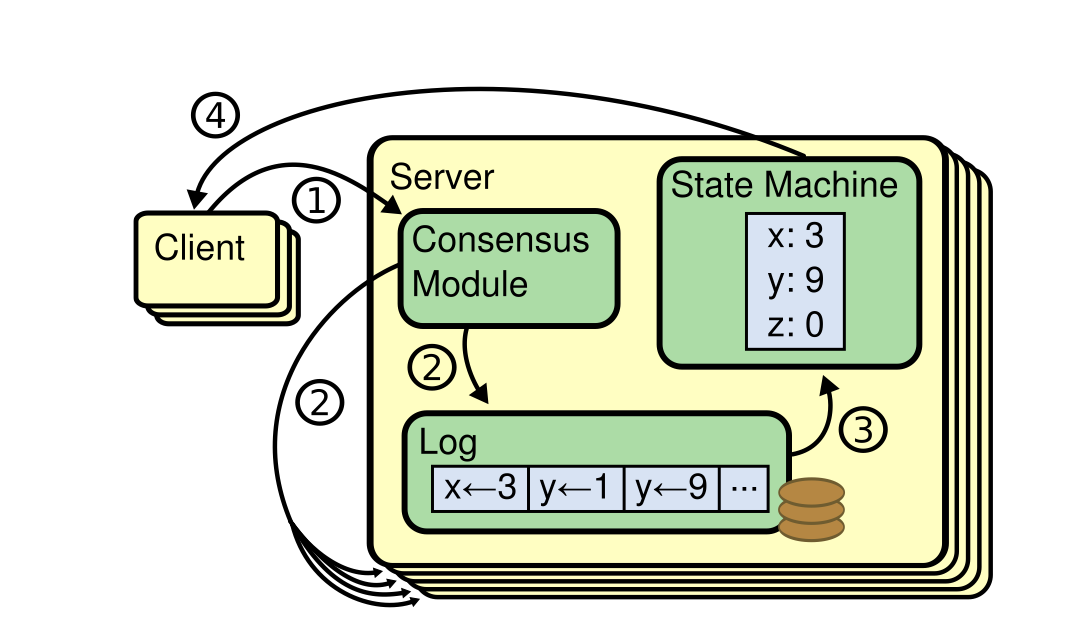
\includegraphics[width=0.7\linewidth]{images/1_replicated_state_machine}
	\caption{Architektur eines replizierten Zustandsautomaten}
	\label{fig:rsm}
\end{figure}

Zu jedem Zeitpunkt ist jeder Knoten in einem von drei möglichen Zuständen sein:

\begin{description} 
	\item[Leader.] Ein Leader verarbeitet alle Client-Anfragen. Wenn ein Client einen Follower kontaktiert, wird er von diesem Follower an den Leader weitergeleitet.
	
	\item[Follower (Anhänger).] Followers sind passiv: sie selber schicken keine Anfragen aus und antworten nur auf mögliche Anfragen des Leader oder eines Kandidaten.
	
	\item[Candidate (Kandidat).] Wenn ein Follower zum Kandidaten wird, darf er sich zum Leader vorschlagen, wobei er vom Quorum aller Knoten unterstützt werden muss.
\end{description}

Im Normalbetrieb es gibt genau einen Leader und alle anderen Knoten sind Followers.

Raft teilt die Zeit in Terms (Amtsperioden) beliebiger Länge. Terms werden mit aufeinanderfolgenden ganzen Zahlen nummeriert. Jeder Term beginnt mit einer Wahl, bei der ein oder mehrere Kandidaten versuchen, Leader zu werden. Wenn ein Kandidat die Wahl gewinnt, fungiert er für den Rest des Terms als Leader. Verschiedene Knoten können die Übergänge zwischen Terms zu verschiedenen Zeiten beobachten. In einigen Situationen übersieht ein Knoten möglicherweise eine Wahl oder sogar ganze Terms. Terms agieren in Raft als eine \textit{"logische Uhr"} und ermöglichen es den Knoten, veraltete Informationen wie z.B. veraltete Leaders zu erkennen. Jeder Knoten speichert eine aktuelle Term-Nummer, die mit der Zeit monoton zunimmt. Der aktuelle Term wird ausgetauscht, wenn Knoten kommunizieren. Ein Term wird gleich nach dem Absturz des aktuellen Leaders beendet.

Um die Verständlichkeit zu verbessern, trennt Raft die Schlüsselelemente des Konsenses:

\begin{description} 
	\item[Wahlprozess des Leaders.] Jeder neu gestartete Knoten wird standardmäßig zum Follower. Ein Knoten bleibt im Follower-Zustand, solange er einen \textit{Heartbeat} von einem Leader erhält. Um eine Wahl zu beginnen, erhöht ein Follower den zuletzt gesehenen Term und wechselt in den Kandidatenzustand. Er stimmt dann für sich selbst und schickt RequestVote-Anfragen parallel an alle anderen Knoten im Cluster. Ein Kandidat bleibt in diesem Zustand, bis eine von drei Optionen vorkommt:
	
	\begin{enumerate}
		\item der Kandidat gewinnt die Wahl
		
		\item ein anderer Knoten etabliert sich als Leader
		
		\item ein Zeitraum vergeht ohne Gewinner
		
		\item ein Kandidat gewinnt eine Wahl, wenn er Stimmen von einem Quorum für denselben Term erhält
	\end{enumerate}
	
	\item[Replikation des Logs.] Sobald ein Leader gewählt wurde, beginnt er mit der Bearbeitung der Client-Anfragen. Jede Client-Anfrage enthält einen Befehl, der von den replizierten Zustandsautomaten ausgeführt werden soll. Der Leader hängt den Befehl als einen neuen Eintrag an sein Log an und schickt AppendEntries-Anfragen zu jedem anderen Knoten, um den Eintrag zu replizieren. Wenn der Eintrag sicher repliziert wurde (d.h. auf einem Quorum aller Knoten), wendet der Leader den Eintrag auf seinen Zustandsautomaten an und gibt das Ergebnis dieser Ausführung an den Client zurück. Jeder Logeintrag enthielt einen Befehl inklusive einer Term-Nummer.
\end{description}

Raft wurde als Basis für folgende Systeme genommen:

\begin{enumerate}
	\item HashiCorp Consul
	
	\item RethinkDB
	
	\item Hazelcast
	
	\item CockroachDB
	
	\item etcd
\end{enumerate}

\subsection{Der Vergleich von Paxos und Raft}

Um die Entscheidung zu treffen, mit welchem Algorithmus ein Produktivsystem implementiert werden soll, muss man sie anhand bestimmter Kriterien vergleichen. Die Algorithmen haben natürlich Ähnlichkeiten aber auch Unterschiede.

\begin{description} 
	\item[Ähnlichkeiten.] Paxos und Raft sind schon deswegen sehr ähnlich, weil sie das Problem des Konsenses in verteilten Systemen lösen, was ein Subproblem des Atomic Broadcasts darstellt (Atomic Broadcasts wird in Probleme des Reliable Broadcasts und Konsenses zerlegt). Beide Algorithmen erfüllen Anforderungen an Safety, Availability und Zeitunabhängigkeit.
	
	Sowohl Paxos als auch Raft versuchen, eine Gesamtreihenfolge von Befehlen zu bestimmen, die auf den replizierten Zustandsautomaten angewendet werden sollen. Diese Algorithmen lösen das gleiche Problem und verfolgen auch den gleichen Ansatz: beide wählen einen Leader, der Befehle in seinen Log hinzufügt und zu einem Quorum repliziert. Wenn ein Leader abstürzt, kommt ein Quorum zusammen und wählt einen neuen Leader. Beide Algorithmen garantieren, dass ein Knoten zum Leader ernannt wird, wenn er Stimmen von einem Quorum aller Knoten erhält. Außerdem haben Paxos und Raft immer nur einen Leader. Im Normalbetrieb hängt der Leader jede Operation an sein Log an und fordert andere Knoten auf, dasselbe zu tun. Sobald ein Quorum das getan hat, markiert der Leader den Logeintrag als \textit{"commited"} (erfolgreich repliziert).
	
	Wenn ein Follower glaubt, dass der Leader abgestürzt ist, wird der Follower zum Kandidaten und ersucht alle anderen Knoten für ihn zu stimmen. Wenn der Kandidat Stimmen von der Mehrheit aller Knoten (Quorum) bekommt, wird er zum Leader. Hier enden die Ähnlichkeiten beider Algorithmen.
	
	
	\item[Technische Unterschiede.] Der größte Unterschied zwischen Paxos und Raft ist, wie die Safety Eigenschaft (always returning a correct result) von Paxos und Raft gewährleistet wird.
	
	In Paxos wird ein Follower für jeden Kandidaten stimmen, der um eine Stimme ersucht. Daher muss die Antwort eines Followers alle bei dem Kandidaten fehlenden Logeinträge enthalten. Der Nachteil dieses Verfahrens ist die Belastung des Netzwerks, wenn ein Follower, der lange Zeit nicht erreichbar war, zu einem Kandidaten wird. Dieser Kandidat wird eine lange Liste von fehlenden Einträgen benötigen, was unter anderem eine langsame Zusammenführung aller fehlenden Einträge zur Folge hat. In Raft seinerseits wird ein Follower nur den Kandidaten anerkennen, der mindestens genauso einen aktuellen Log hat, wie der Follower. Generell wollte der Erfinder des Raft-Algorithmus die Einfachheit auf zwei Arten erreichen: die Anzahl von Nachrichten zu reduzieren und den Wahlprozess zu optimieren.
	
	In der Abbildung \ref{fig:logstate} wird ein Cluster mit fünf Knoten abgebildet. Der Knoten 1 ist der Leader, der Knoten 4 (mit einem einzelnen Eintrag im Log) ist ein Follower, der eine lange Zeit keine Updates von dem Leader erhalten hat. Laut dem Paxos-Algorithmus kann der vierte Follower auch zum Leader gewählt werden. Wenn er tatsächlich zum Leader gewählt wird, muss er alle fehlenden Logeinträge anordnen. Laut Raft also entweder der dritte oder fünfte Knoten. Nur diese beiden Knoten haben einen Log, der zumindestens genauso aktuell ist, wie der Log bei einem Quorum aller Knoten.
	
	\begin{figure}
		\centering
		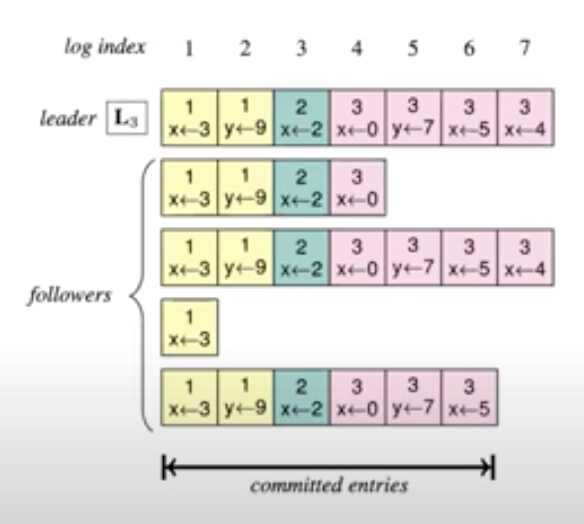
\includegraphics[width=0.7\linewidth]{images/2_log_state}
		\caption{Zustand eines Logs.}
		\label{fig:logstate}
	\end{figure}
	
	
	\item[Nicht technische Unterschiede.] Wenn man den Inhalt der ursprünglichen Publikation der Paxos- und Raft-Algorithmen vergleicht, wirkt der Raft-Algorithmus deutlich verständlicher und einfacher zu implementieren. Darauf hat der Autor des Raft-Algorithmus mehrmals hingedeutet. Das wurde auch durch eine Reihe von Publikationen bestätigt (Paxos Made Simple, Paxos Made Moderately Complex, Paxos Made Live), die versucht haben, den ursprünglichen Paxos-Algorithmus simpler zu erläutern. Es ist erwähnenswert, dass die erste von diesen Publikationen vom Autor des Paxos Algorithmus verfasst wurde.
\end{description}

Die Praxisorientiertheit und der Pragmatismus von Raft werden auch durch die Erwähnung bestimmter Technologien für den Nachrichtenaustausch hervorgehoben. Diese Technologie nennt sich \textit{RPC} (Remote Procedure Call). In der Publikation des Paxos-Algorithmus gibt es keine solchen Tipps.

Der Vergleich in der Tabelle \ref{tab:vergleich} zeigt deutlich, dass Raft durch seine Erklärbarkeit und pragmatische Darstellung einen frischen Blick auf moderne verteilte Systeme wirft und die Optimierung der Replikation eine bessere Option für ein Produktivsystem darstellt. Das wird auch durch seine in den letzten Jahren schnell gestiegene Popularität bei großen kommerziellen Projekten (z.B. HashiCorp Consul) bestätigt.

\begin{table} \centering
	\begin{tabular}{|p{5cm}|p{5cm}|p{5cm}|} 
		
		\hline
		&  \textbf{Raft} & \textbf{Paxos}\\
		
		\hline
		Veröffentlichung & 2014 & 1998\\
		
		\hline
		Erklärbarkeit des Algorithmus in der ursprünglichen Publikation laut dem Raft Artikel & Sehr gut & Mittelmäßig\\
		
		\hline
		Erklärbarkeit des Kerns des Algorithmus laut dem Raft Artikel  & Gut & Gut\\
		
		\hline
		Spielraum bei der Implementierung & Weniger Spielraum. Einfach zu implementieren. & Mehr Spielraum. Viele Annahmen müssen getroffen werden.\\
		
		\hline
		Gewährleistung der Safety Eigenschaft & Nur der Kandidat mit dem aktuellsten Stand des Logs wird gewählt. Optimale Nutzung der Netzwerk Ressourcen. & Jeder Kandidat darf gewählt werden. Zusendung fehlender Logeinträge ist erforderlich. Nutzung der Netzwerkressourcen ist nicht optimal.\\
		
		\hline
	\end{tabular}
	\caption{Vergleich der Raft und Paxos Algorithmen}
	\label{tab:vergleich}
\end{table}

\section{Concurrency Modelle für die Umsetzung von verteilten Systemen}




















\begin{description} 
	\item[.] 
	
	\item[.] 
	
	\item[.] 
\end{description}

\begin{enumerate}
	\item 
	
	\item 
	
	\item 
	
	\item 
\end{enumerate}
\chapter{Entwicklung}
\label{cha:Entwicklung}


\chapter{Fazit}
\label{cha:Fazit}

Ziel der vorliegenden Bachelorarbeit war es, durch die Analyse von Concurrency Modellen und Algorithmen für verteilte Systeme eine optimale Kombination von theoretischen und praktischen Ansätzen zur Entwicklung der Software für unbemannter Luftfahrzeugen genauer zu beleuchten. Für die Beantwortung dieser Frage wurde eine Studie zu den am häufigsten verwendeten Algorithmen für verteilte Systeme, Concurrency Modelle sowie Concurrency Frameworks durchgeführt.

Die Ergebnisse der Untersuchung der Algorithmen für verteilte Systeme haben ergeben, dass Raft-Algorithmus mit seiner Erklärbarkeit und Protokoll-Effizienz die beste Option für die Entwicklung des Konsensmoduls darstellt. Der Vergleich mit den alternativen Algorithmen hat deutlich gezeigt, dass Raft mit seiner pragmatischen Darstellung und seinem frischen Blick auf Replikationsverfahren den Paxos-Algorithmus hinter sich lässt. Diese Tatsache wird auch dadurch bestätigt, dass die Popularität des Algorithmus in letzten Jahren sehr schnell gestiegen ist.

Ein anderer wichtigster Aspekt, der bei der Entwicklung verteilter Systeme berücksichtigt sein muss, ist Concurrency. Verteilte Systeme stellen eigene Anforderungen an Concurrency Modell. Unter anderem sind Fehlertoleranz, bidirektionale Kommunikation und reibungsloser Aufruf von Remote-Services dafür wichtig. Durch den Vergleich von vier populärsten Concurrency Modelle (Aktormodell, CSP, funktionale Programmierung, Threads und Mutex) wurde der Schluss gezogen, dass Aktormodell für die Erfüllung der erwähnten Anforderungen an die Software für Drohnen am besten geeignet ist. 

Praktischer Teil der Arbeit hat die Implementierung des Raft-Algorithmus mit der Programmiersprache Scala umgefasst. Die Implementierung hat gezeigt, dass solche funktionale Programmiersprachen wie Scala mit ihren fortgeschrittenen Pattern-Matching Eigenschaften den Zeitaufwand beim Testing und auch bei der Entwicklung sparen. Aus diesen Befunden kann darauf geschlossen werden, dass der Raft-Algorithmus in der Kombination mit dem Aktormodell die Rahmenbedingungen der verteilten Systeme in unbemannten Luftfahrzeugen erfüllt. 


%%%----------------------------------------------------------
\appendix                                            % Anhang 
%%%----------------------------------------------------------

\chapter{Technische Informationen}
\label{app:TechnischeInfos}

	% Technische Ergänzungen
\chapter{Ergänzende Inhalte} % \chapter{Inhalt der CD-ROM/DVD}
\label{app:materials}


Auflistung der ergänzenden Materialien zu dieser Arbeit, die zur digitalen Archivierung an der 
Hochschule eingereicht wurden (als ZIP-Datei).

% Nur als Beispiel, die Struktur sollte man an die eigenen Bedürfnisse anpassen!

\section{PDF-Dateien}
\begin{FileList}{/}
\fitem{thesis.pdf} Finale Master-/Bachelorarbeit (Gesamtdokument)
\end{FileList}

\section{Mediendaten}
\begin{FileList}{/media}
\fitem{*.ai, *.pdf} Adobe Illustrator-Dateien
\fitem{*.jpg, *.png} Rasterbilder
\fitem{*.mp3} Audio-Dateien
\fitem{*.mp4} Video-Dateien
\end{FileList}


\section{Online-Quellen (PDF-Kopien)}
\begin{FileList}{/online-sources}
\fitem{Reliquienschrein-Wikipedia.pdf} \citenobr{WikiReliquienschrein2018}
\end{FileList}



	% Inhalt der CD-ROM/DVD
\chapter{Fragebogen}
\label{app:Fragebogen}

	% Chronologische Liste der Änderungen
\chapter{\latex-Quellcode}
\label{app:Quellcode}

	% Quelltext dieses Dokuments

%%%----------------------------------------------------------
\MakeBibliography                        % Quellenverzeichnis
%%%----------------------------------------------------------

%%% Messbox zur Druckkontrolle ------------------------------
\chapter*{Messbox zur Druckkontrolle}



\begin{center}
{\Large --- Druckgröße kontrollieren! ---}

\bigskip

\calibrationbox{100}{50} % Angabe der Breite/Hoehe in mm

\bigskip

{\Large --- Diese Seite nach dem Druck entfernen! ---}

\end{center}



%%%----------------------------------------------------------
\end{document}
%%%----------------------------------------------------------